\section{Long Short-Term Memory (LSTM)}

As mentioned in \textbf{\autoref{rnn1}}, there are different types of \gls{rnn}s, but the \gls{lstm} model is one of the most widely used with regards to \gls{ips}. We will therefore also use the \gls{lstm} structure for our experiment with \gls{rnn}.

In a recurrent network, the output from a previous step will be used as input for the next step. In an \gls{lstm} model, the nodes are recurrent, and they also include a cell state. This cell state is the working memory space which is used by the node, so the information can be stored and retrieved over multiple time steps. Therefore, in an \gls{lstm}, the input value, the previous output, and the cell state are all used in the calculations of the node. The results of this calculation are used to get an output value, but also to update the cell state. Besides having parameters for defining how inputs should be used in the calculations, as in standard neural networks, the \gls{lstm}'s nodes also include gates. The gates are responsible for controlling the flow within the node, which especially includes determining how much of the saved information should be used in a given calculation. The gate parameters are made of weights and biases, and therefore, the input determines the behaviour. There are three types of gates in an \gls{lstm} network; the input gate, the forget gate and the output gate. The \gls{lstm} network can therefore be divided into three different parts, as shown in \textbf{\autoref{fig:lstm}}. 

\begin{figure}[H]
    \centering
    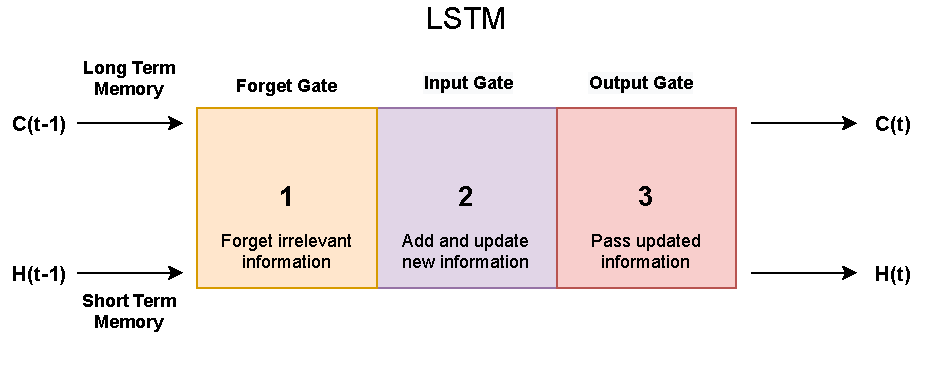
\includegraphics[scale=0.85]{Images/Experiments/lstm.pdf}
    \caption{Overview of an LSTM network.}
    \label{fig:lstm}
\end{figure}

In the first part of \gls{lstm}, the network will try to determine whether the information from the previous timestamp is relevant or if it should be forgotten. In the second part, the cell will try to learn new information from the given input, and update the information. In the last step, the cell will pass the information that it has updated from the current timestamp to the next timestamp. Besides from the cell state, the \gls{lstm} network also includes a hidden state, as known in standard \gls{rnn} networks. In \textbf{\autoref{fig:lstm}}, $H(t-1)$ denotes the hidden state of the previous timestamp, and $H(t)$ denotes the hidden state of the current timestamp. $C(t-1)$ and $C(t)$ denote the previous and current timestamps for the cell state, respectively. The cell state can be viewed as the long term memory of the system, and the hidden state can be seen as the short term memory. The information from the timestamps are used in the calculations in the different gates in the network.\cite{lstmVidhya}

The \gls{lstm} networks are less exposed to the vanishing gradient problem, mentioned in \textbf{\autoref{sec:vanishing_exploding_gradient_problem}}, but the exploding gradient problem can still be encountered. Another disadvantage of the \gls{lstm} is that they are very computational intensive.\cite{Yalcın2021}